\documentclass[10pt,a4paper]{article}
\usepackage[margin=2.2cm]{geometry}
\usepackage{fontspec}
\usepackage{kotex}
\setmainfont{Apple SD Gothic Neo}
\setsansfont{Apple SD Gothic Neo}
\usepackage{amsmath,amssymb}
\usepackage{graphicx}
\usepackage{booktabs}
\usepackage{caption}
\usepackage[dvipsnames]{xcolor}
\usepackage[colorlinks=true,linkcolor=MidnightBlue,citecolor=MidnightBlue,
            urlcolor=MidnightBlue]{hyperref}
\usepackage{titlesec}
\titleformat{\section}{\large\bfseries}{\thesection}{0.6em}{}
\titleformat{\subsection}{\normalsize\bfseries}{\thesubsection}{0.5em}{}
\captionsetup{font=small,labelfont=bf}
\setlength{\parskip}{0.35em}
\setlength{\parindent}{0pt}

\usepackage{mdframed}
\newmdenv[linewidth=0.4pt,linecolor=gray!60,backgroundcolor=gray!5,
          innertopmargin=6pt,innerbottommargin=6pt,skipabove=8pt,skipbelow=8pt]{claimbox}
\newcommand{\claim}[2]{\begin{claimbox}\textbf{주장.} #1\par\smallskip
  \textcolor{gray!70}{\textbf{반증 조건.} #2}\end{claimbox}}

\title{\bfseries 인코더가 아니라 원료다\\[2pt]
\large 임베딩 병기, 제목 수준에서 기각 --- 세 번째 확인}
\author{월드모델 실험실 · 노트 $805$}
\date{2026-08-07}
\begin{document}\maketitle

\section{한 줄}

로드맵 A$1$(\emph{동결 임베딩을 축에 병기하면 통계 레인에 텍스트가 공급된다})을
챌린저 레인에서 쟀다 --- MiniLM 다국어 $\to$ \textbf{PCA$8$(학습만 · 노트 $645$)}
$\to$ TabPFN concat. 제목이 판 행과 정렬되는 셋(시장팝업·도서·게임)만.
\textbf{배선에서 아이돌($81$ 대 $173$)·팝업($75$ 대 $89$)의 어긋남을 잡아 미리
뺐다.}

\begin{center}
\begin{tabular}{lrrrrl}
\toprule
& A 기준 & B 병기 & B$-$A & 문턱 & 판정 \\
\midrule
시장팝업 & $0.2341$ & $0.2985$ & $+0.0644$ & $0.1543$ & \textbf{모} \\
도서 & $0.1704$ & $0.1311$ & $\mathbf{-0.0394}$ & $0.0346$ & \textbf{해} \\
게임 & $0.5371$ & $0.5206$ & $-0.0165$ & $0.0704$ & 없 \\
\bottomrule
\end{tabular}
\end{center}

\textbf{(좋)이 하나도 없다 --- A$1$ 을 제목 수준에서 기각한다.} 규약 $45$ 의 네
방향 갈래가 이번엔 처음부터 있었고, 실측이 셋 다 다른 갈래로 갔다.

\begin{figure}[t]\centering
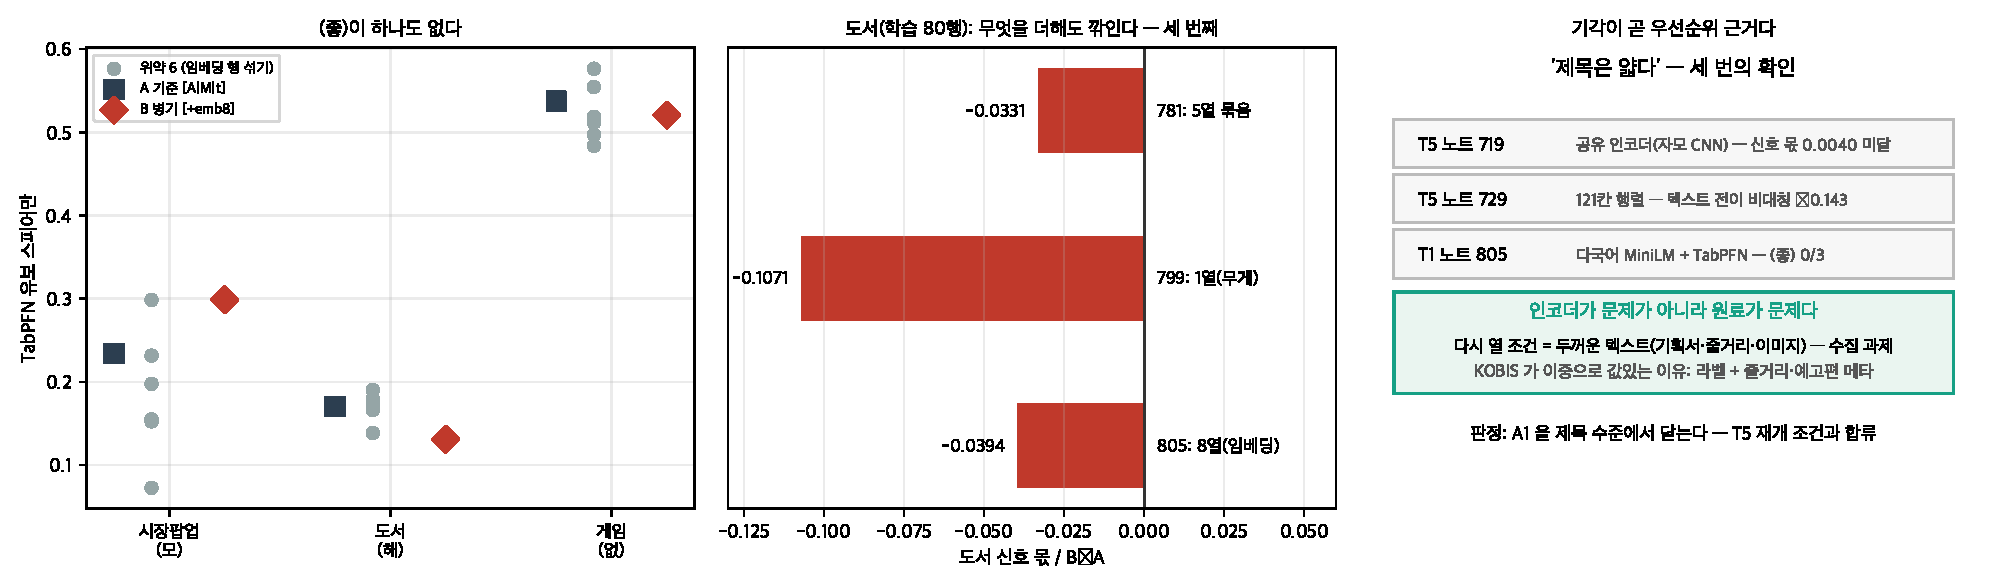
\includegraphics[width=0.99\textwidth]{figs/thin.pdf}
\caption{왼쪽: 세 도메인의 A·B·위약. 가운데: \textbf{도서는 무엇을 더해도
깎인다} --- 세 번째. 오른쪽: ``제목은 얇다''의 세 확인.}
\end{figure}

\section{도서가 또 ``해''다 --- 그리고 시장팝업의 위약이 사납다}

\claim{\textbf{도서($80$ 학습행)는 내용과 무관하게 열을 더하면 깎인다} --- $5$열
묶음 $-0.0331$(논문 $155$) · $1$열 무게 $-0.1071$(논문 $163$) · $8$열 임베딩
$-0.0394$(이번). 세 번 다 다른 내용, 같은 방향. \textbf{행이 열을 못 이기는
도메인이 있고, 그 문턱은 내용이 아니라 행수다.}}
{시장팝업의 부수 발견이 경고다 --- \textbf{무작위 $8$열이 이 도메인을
$0.073{\sim}0.298$ 로 흔든다}(뽑기 SD $0.077$). B($0.2985$)가 위약 최대($0.2984$)를
$0.0001$ 차로 넘어 ``위약 전부보다 큼''이 문자로는 참이지만 \textbf{사실상
동률이다.} 이 도메인의 챌린저 측정은 열 추가 실험에 취약하고, 앞으로 이 폭을
선반영해야 한다.}

\section{세 번째 확인 --- 인코더가 아니라 원료다}

T$5$ 가 두 번 쟀다: 공유 인코더 신호 몫 $0.0040$ 미달(노트 $719$) · $121$칸 행렬
비대칭 $-0.143$(노트 $729$). 이번엔 \textbf{다른 인코더}(다국어 MiniLM)와
\textbf{다른 레인}(TabPFN)에서 같은 답이다.

\claim{\textbf{``제목은 얇다''는 이제 아키텍처 독립적 결론이다.} Qwen$3$-$4$B
선발 비교는 무의미해졌다 --- 인코더를 키워도 제목에 없는 정보는 안 나온다.
\textbf{다시 열 조건은 T$5$ 와 합류한다}: 두꺼운 텍스트(기획서 원문 · 줄거리 ·
이미지). 그것은 수집 과제이고, \textbf{KOBIS 가 이중으로 값있는 이유가 여기
있다} --- 라벨(일별 관객)과 함께 줄거리·예고편 메타가 온다.}
{제목 $384$차원을 PCA$8$ 로 눌렀다 --- \textbf{압축이 신호를 죽였을 가능성}은
남는다. 다만 $8$차원을 고른 이유가 규약 $39 \cdot 641$(얇은 레짐 열 예산)이고,
차원을 늘리는 쪽은 도서·게임에서 이미 (해)·(없)이 더 깊어지는 방향이다 ---
넓혀서 살아날 그림이 아니다.}

\section{예측 채점과 처분}

기각 확률 $2/3$ 로 적었고 실현됐다. (해)의 도메인만 틀렸다 --- 게임($20\%$)이
아니라 \textbf{더 얇은 도서}가 먼저 깎였다. \textbf{처분}: A$1$ 닫음(제목 수준) ·
T$1$ 다음은 \textbf{아이돌 축 배선 수리 후 챌린저 재검}(논문 $168$ 의 선행 시험) ·
판 $\rho$ $0.4689$ 그대로.

\end{document}
